\chapter{Laser Cutting}
Laser cutting is split into three groups:
\begin{itemize}
    \item Gas assisted cutting \pd fusion and flame cutting
    \item Remote fine cutting
    \item Sublimation cutting
\end{itemize}

\section{Gas assisted cutting}

Figure \ref{fig:gcutinghead} show a nozzle and its parts for gas assisted cutting. 
\begin{figure}[h!]
    \centering
    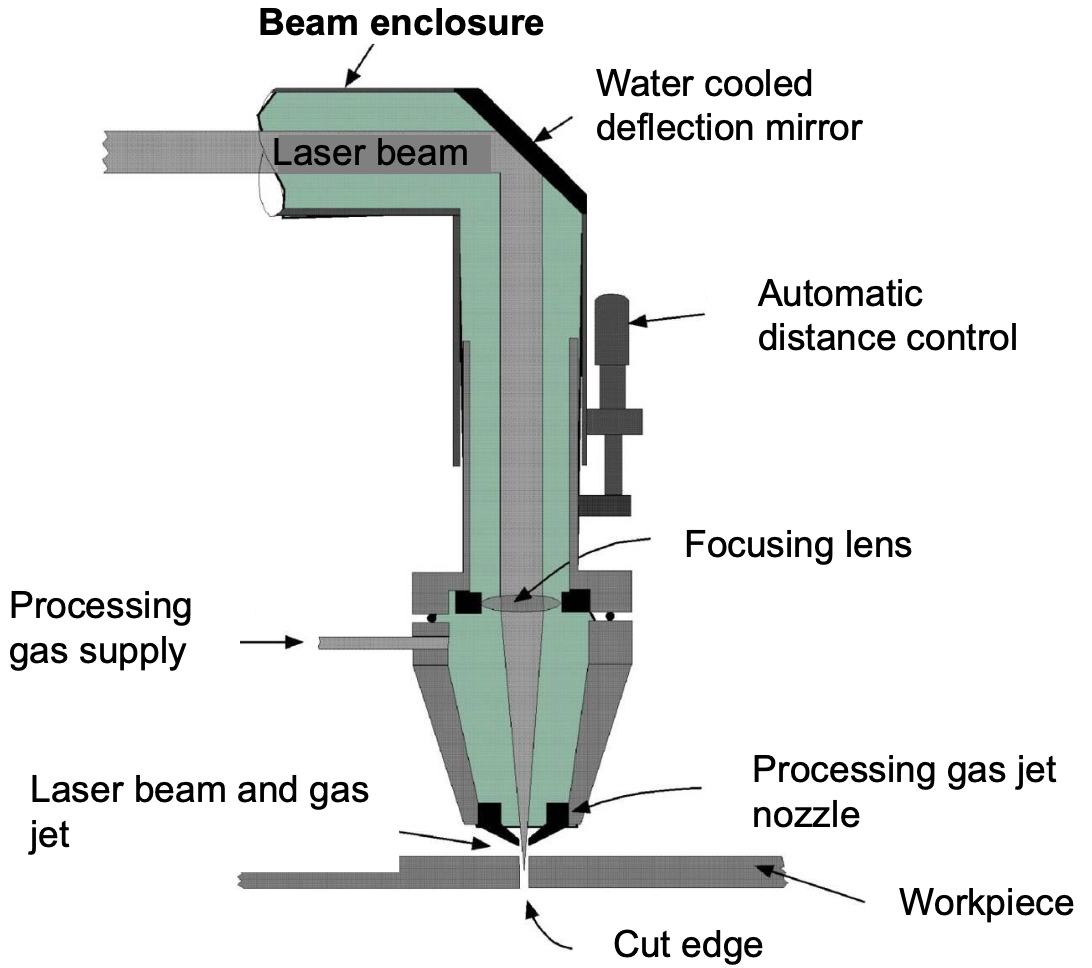
\includegraphics[width=0.5\textwidth]{slike/gasnozzle.png}
    \caption{Cutting head for gas assisted cutting. \sln}
    \label{fig:gcutinghead}
\end{figure}

Cutting is achieved by:
\begin{itemize}
    \item Melting and melt removal, by gas jet. Intensity \pd $10^5 \frac{W}{cm^2}$.
    \item Melt removal by melt overflow. Intensity \pd $10^6 \frac{W}{cm^2}$.
    \item Direct evaporation or sublimation. Intensity \pd $10^7 \frac{W}{cm^2}$
\end{itemize}

Gas is used for preventing oxidization ($N_2, Ar \dots$) or initializing oxidization ($O_2$).
\textit{Flame cutting} is oxygen assisted, inert gasses are used for \textit{fusion}
and \textit{sublimation} cutting. 

\subsection{Fusion cutting}
Laser melts material, which is mechanically ejected by the gas jet from the bottom of the \textbf{kerf}. Gas is inert and 
pressurized to $2-20$ bar. 

\subsection{Flame cutting}
Flame cutting utilizes strong exothermal reaction between oxygen and the metal workpiece, which then burns \pd flame cutting.
Laser heats metal to high temperature to enable reaction with $O_2$. Chemical reaction with oxygen is the main source of energy.
Energy from this reaction heats and melts the combustion products so that the blow-off of melt and liquid reacts with the $O_2$ jet.
Surrounding material is heated and melted, edges oxidize.

Cutting speed depends on the thickness of material, shown on figure \ref{fig:cspeed}, where $v \left[\frac{m}{min}\right]$ is the
cutting speed and $s [mm]$ is the material thickness. 
\begin{figure}[h!]
    \centering
    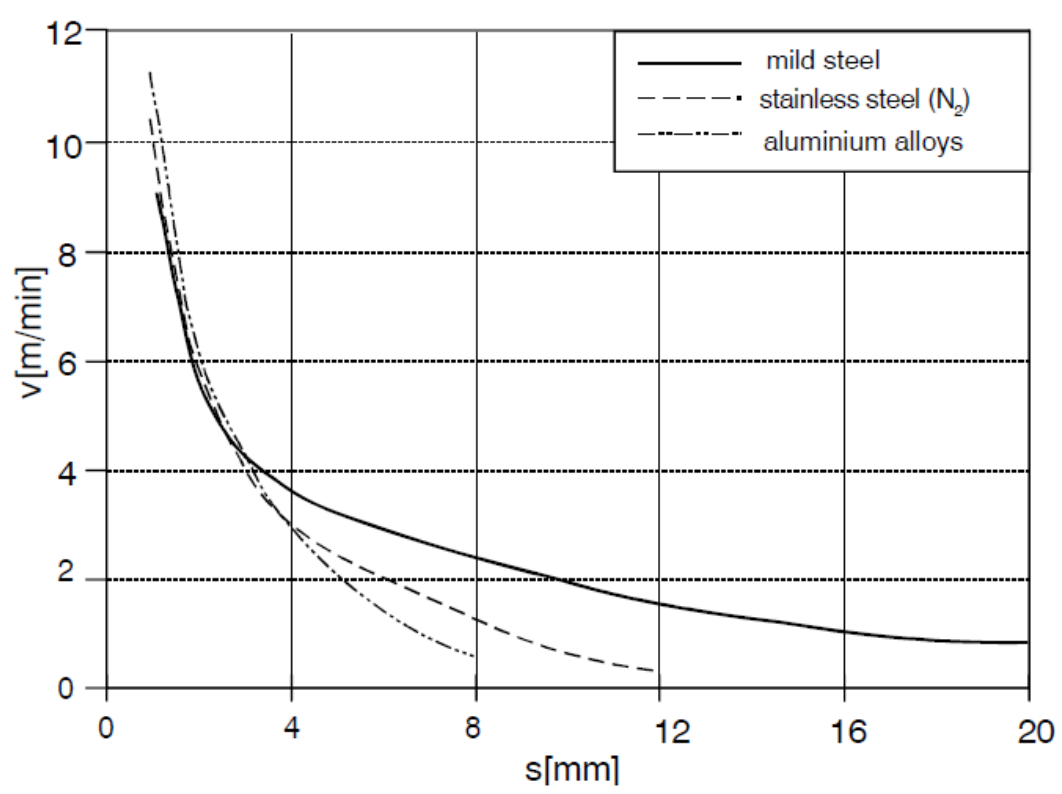
\includegraphics[width=0.5\textwidth]{slike/cspeed.png}
    \caption{Cutting speed. \sln}
    \label{fig:cspeed}
\end{figure}


\subsection{Comparison between Fusion and Flame cutting}

\begin{table}[h!]
    \begin{tabular}{|l|l|l|}
    \hline
     &
      Fusion cutting &
      Flame cutting \\
      \hline
    Pros: &
      \begin{tabular}[c]{@{}l@{}}Fusion cutting is used for \\ cutting metals  and other fusible \\ materials. There is no oxidation \\ due to inert assist gas\end{tabular} &
      \begin{tabular}[c]{@{}l@{}}High processing speed.\\ Can cut thick material.\end{tabular} \\
    \hline
    Cons: &
      \begin{tabular}[c]{@{}l@{}}Laser must supply all the energy.\\ Piercing is more difficult\end{tabular} &
      \begin{tabular}[c]{@{}l@{}}Material must react with \\ oxygen at high temperature.\\ Kerf edges oxidize. \\ Oxide layer must be removed prior\\ to painting or powder coating.\end{tabular} \\
    \hline

    \end{tabular}
    \end{table}


\section{Lasers for cutting}
Lasers used for flame and fusion cutting are $CO_2$ or $Nd$ doped lasers.
The $CO_2$ laser is usable for many materials due to their  absorptivity at the $10.6 \mu m$. Such materials are glass, plastic, wood, cardboard\dots

$Nd$ doped fiber and solid lasers with $\lambda = 1 \mu m$ are used for cutting steel, copper based alloys and precious metals.
Beam of a $Nd$ doped laser can be guided using an optical fiber, $CO_2$ laser beam can't be used with optical fiber.

For cutting, CW lasers with high power (kW) and circularly polarized high quality beam are perfered. 

\section{Influence of polarization}
Polarization influences absorptivity, shown on figure \ref{fig:cpolabs}. 

\begin{figure}[h!]
    \centering
    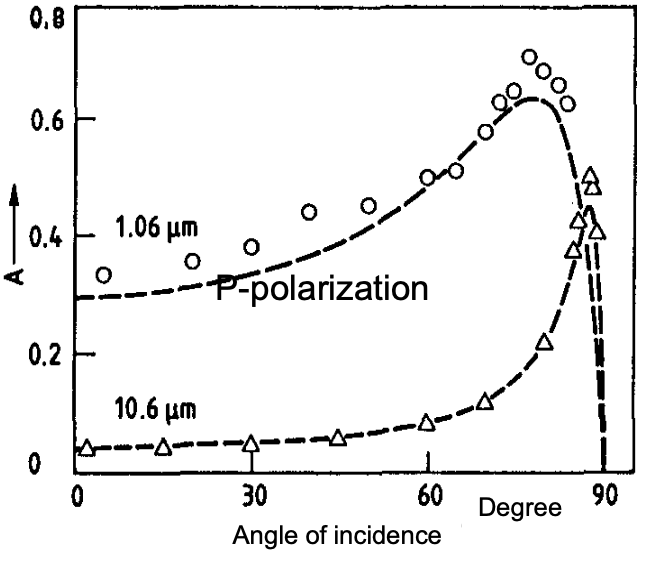
\includegraphics[width=0.5\textwidth]{slike/cpolabs.png}
    \caption{$CO_2$ and $Nd:YAG$ absorptivity comparison. \sln}
    \label{fig:cpolabs}
\end{figure}

Angle of incidence influences the optimum feed and speed for given material thickness and laser power. We have to 
avoid the \textit{Brewster's angle}.
When the cut is curved, the polarization has to be changed according to the cutting direction or a  \textit{circularly polarized} laser can be used. 

\section{Remote fine cutting}

With remote fine cutting, a scanner head is used. It enables higher speed and provides better accessibility to the workpiece. 
Remote fine cutting does not use cutting gas, recoil pressure of the vapour expels the melt.

Parameters are given in table \ref{tab:schparm}
\begin{table}[h!]
    \centering
    \begin{tabular}{|c|c|}
        \hline
        Parameter & Value \\
        \hline
        Thickness & $< 1 mm$ \\
        \hline
        Intensity & $0.5 - 1 \frac{MW}{mm^2}$\\
        \hline
        Speed & $> 100 \frac{m}{min}$ \\
        \hline
        Multi pass & $50-100 \mu m$ \\
        \hline

    \end{tabular}
    \caption{Parameters}
    \label{tab:schparm}
\end{table}

\section{Sublimation/vaporization cutting}

Sublimation cutting is used with materials \textit{without} a distinct melting point, such as wood, textile, paper \dots
Material is vaporized not melted, process gas ($Ar, N_2, HE$) is added to shield it from oxygen.
Sublimation cutting reduces the HAZ and melt pool. Laser beam has to have high intensity and good beam quality. 
Cutting speed is low.
